\documentclass[a4paper,11pt,fleqn]{article}%fleqn pour aligner les equations à gauche
\usepackage{../../Styles/Exercice}


\newcommand{\chnum}{Chapitre 12}
\newcommand{\chtitle}{Mouvement dans un champ uniforme}
\newcommand{\dtype}{Exercices}
  
  
\begin{document}
\maketitle

\begin{multicols}{2}
\section{L'expérience de Scott}
	\begin{minipage}{.47\textwidth}
	Lors de la mission Apollo 15, en 1971, les astronautes séjournent sur la Lune durant près de 64 heures et y réalisent différentes expériences. Peu avant la fin de la mission, David Scott prend dans chaque main une plume et un marteau afin de vérifier la loi de la chute des corps de Galilée. il les lâche au même instant : la plume et le marteau touchent le sol lunaire simultanément, \SI{1,2}{\second} plus tard.\\
L'axe ($Oz$) est dirigé vers le bas et son origine $O$ est confondue avec le centre de masse du marteau à l'instant du lâcher.
	\end{minipage}

	\begin{minipage}{.47\textwidth}
	\begin{center}
	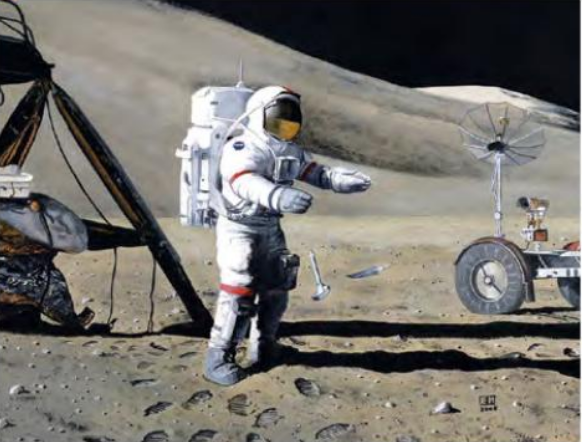
\includegraphics[scale=.3]{Ressources/TSPE_C5_Ex_Fig1.png}
	\end{center}
	\end{minipage}

\begin{enumerate}
	\item Préciser le référentiel d'étude.
	\item Appliquer la deuxième loi de Newton à chaque objet et montrer qu'ils ont le même vecteur accélération.
	\item En déduire l'expression de la composante verticale $v_Z(t)$, puis celle de $z(t)$.
	\item Exprimer $g_L$, l'intensité de pesanteur sur la Lune, en fonction du temps de chute $t_c$ et de la hauteur de chute $h$.
	\item Utiliser le document fourni pour estimer $h$, et en déduire la valeur de $g_L$.
	\item La valeur de $g_L$ est en réalité de \num{1,61} \unit{\newton \per \kilo \gram}. Commenter l'éventuel écart constaté.
\end{enumerate}
\textbf{Donnée :}
\begin{itemize}
	\item \textbf{Taille de Davis Scott :} $l =$ \num{1,84} \unit{\meter}
\end{itemize}
\section{Détermination d'une vitesse initiale}
	\begin{minipage}{.47\textwidth}
		Avant de réaliser  un service, une joueuse de tennis lance sa balle verticalement vers le haut. Son point de lancement est pris comme origine d'un axe vertical dirigé vers le haut. On assimile la balle à son centre de masse $G$.
	\end{minipage}
	\begin{minipage}{.5\textwidth}
		\begin{center}
			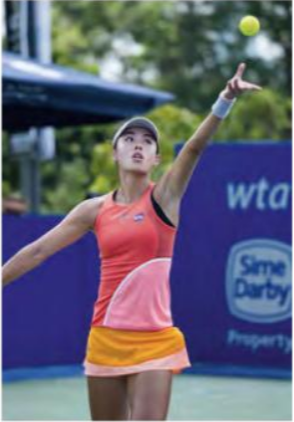
\includegraphics[scale=.3]{Ressources/TSPE_C5_Ex_Fig2.png}
		\end{center}
	\end{minipage}
\begin{enumerate}
	\item Établir l'expression de la composante $v_z(t)$ de la vitesse de la balle.
	\item Établir l'équation horaire $z(t)$ du mouvement de la balle.
	\item Calculer la valeur de la vitesse initiale que la joueuse soit communiquer à la balle si elle veut qu'elle s'élève de \num{2,0} \unit{\meter} par rapport à sa position initiale.
\end{enumerate}

\section{Représentation des équations horaires}
Lors d'une séance de travaux pratiques, des élèves ont travaillé sur la vidéo d'un tir au but et réalisé le pointage. Ils ont ensuite tracé les équations horaires du mouvement du centre de masse du ballon, $x(t)$ et $y(t)$, puis obtenu et tracé $v_x(t)$ et $v_y(t)$. Contents de leur travail, ils ont imprimé les graphiques obtenus ... sans indiquer les noms et les unités des axes !\\
Afin de les aider, leur professeur leur rappelle que :
\begin{eqnarray}
	\vec{v} \left\lbrace \begin{aligned}
	v_x(t) = v_0 \cdot \cos(\alpha)\\
	v_y(t) = -g \cdot t	+ v_0 \cdot \sin(\alpha)
	\end{aligned} \right\rbrace _{(O,\vec{i},\vec{j})} \nonumber
\end{eqnarray}
\begin{enumerate}
	\item Déterminer les expressions de $x(t)$ et $y(t)$.
	\item Associer chaque graphique à l'équation correspondante.
\end{enumerate}
\begin{tikzpicture}[scale=.9,transform shape]
	\draw[-Stealth] (0,0) to (4.5,0);
	\draw[-Stealth] (0,0) to (0,3.5);
	
	\foreach \k in {1,...,4} {
		\draw (\k,0) -- (\k,-.1);
		\pgfmathsetmacro{\lk}{\k/2}
		\draw (\k,0) node[below] {\lk};
		}
	\foreach \x in {1,...,8} {
		\draw (-.1,3/8*\x) -- (0,3/8*\x);
		\draw (0.3*\x,0.3*1.1*\x) node {$+$};
		}
	\foreach \x in {0,2,4,6,8} {
		\draw (-.1,3/8*\x) node[left] {\x};
	}
	\draw [domain=0:3] plot(\x,{1.1*\x});
\end{tikzpicture}
\begin{tikzpicture}[scale=.9,transform shape]
	\draw[-Stealth] (0,0) to (4.5,0);
	\draw[-Stealth] (0,0) to (0,3.5);
	
	\foreach \k in {1,...,4} {
		\draw (\k,0) -- (\k,-.1);
		\pgfmathsetmacro{\lk}{\k/2}
		\draw (\k,0) node[below] {\lk};
		}
	\foreach \x in {1,...,8} {
		\draw (-.1,3/8*\x) -- (0,3/8*\x);
		}
	\foreach \x in {.25,.5,...,3.5} {
		\draw (\x,-0.5*\x^2+2.5*\x) node {$+$};
		}
	\foreach \x in {0,2,4,6,8} {
		\draw (-.1,3/8*\x) node[left] {\x};
	}
	\draw [domain=0:3.5] plot(\x,{-0.5*\x^2+2.5*\x});
\end{tikzpicture}

\noindent \begin{tikzpicture}[scale=.9,transform shape]
	\draw[-Stealth] (0,0) to (4.5,0);
	\draw[-Stealth] (0,0) to (0,3.5);
	
	\foreach \k in {1,...,4} {
		\draw (\k,0) -- (\k,-.1);
		\pgfmathsetmacro{\lk}{\k/2}
		\draw (\k,0) node[below] {\lk};
		}
	\foreach \x in {1,...,8} {
		\draw (-.1,3/8*\x) -- (0,3/8*\x);
		}
	\foreach \x in {.25,.5,...,3.5} {
		\draw (\x,2.5) node {$\times$};
		}
	\foreach \x in {0,2,4,6,8} {
		\draw (-.1,3/8*\x) node[left] {\x};
	}
	\draw [domain=0:3.5] plot(\x,2.5);
\end{tikzpicture}
\begin{tikzpicture}[scale=.9,transform shape]
	\draw[-Stealth] (0,0) to (4.5,0);
	\draw[-Stealth] (0,-1.75) to (0,1.75);
	
	\foreach \k in {1,...,4} {
		\draw (\k,0) -- (\k,-.1);
		\pgfmathsetmacro{\lk}{\k/2}
		\draw (\k,0) node[below] {\lk};
		}
	\foreach \x in {-4,...,4} {
		\draw (-.1,3/8*\x) -- (0,3/8*\x);
		}
	\foreach \x in {.25,.5,...,3.5} {
		\draw (\x,-.75*\x+1.5) node {$+$};
		}
	\foreach \x in {-4,-2,...,4} {
		\draw (-.1,3/8*\x) node[left] {\x};
	}
	\draw [domain=0:3.5] plot(\x,{-.75*\x+1.5});
\end{tikzpicture}

\section{Accélération d'un électron}
Un faisceau d'électrons est émis dans le vide par un filament avec une vitesse initiale négligeable. Il est accéléré par une tension $U$ de valeur absolue \SI{200}{\volt} appliquée entre deux plaques A et B. La distance entre les plaques est $d$ = \SI{4,0}{\centi\meter} La plaque B est percée d'un trou noté $O$.\\
\begin{center}
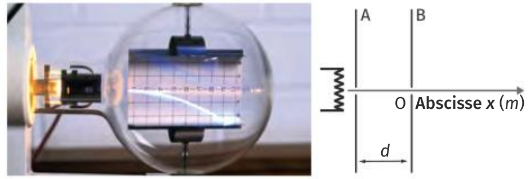
\includegraphics[scale=.5]{Ressources/TSPE_C5_Ex_Fig4.png}
\end{center}
\begin{enumerate}
	\item Préciser le signe de la tension $U$ pour que l'électron soit accéléré.
	\item Exprimer la valeur et préciser la direction et le sens du champ électrique $\vec{E}$ régnant entre les plaques A et B.
\end{enumerate}
On considère qu'une force est négligeable devant une autre si son intensité est au moins \num{1E3} fois plus petite.
\begin{enumerate}[resume]
	\item Montrer que le poids de l'électron est négligeable devant la force électrique.
	\item Calculer la vitesse de l'électron lorsqu'il arrive au point $O$.
\end{enumerate}
\textbf{Données :}
\begin{itemize}
	\item \textbf{Intensité de pesanteur :} $g $ = \SI{9,81}{\newton \per \kilo \gram}
	\item \textbf{Masse de l'électron :} $m_e$ = \SI{9,11E-31}{\kilo \gram}
	\item \textbf{Charge élémentaire :} $e$ = \SI{1,60E-19}{\coulomb}
\end{itemize}

\section{Déviation d'une particule}
\begin{minipage}{.27\textwidth}
Une particule chargée positivement pénètre dans un champ électrique uniforme créé entre les plaques d'un condensateur plan. Sur la figure ci-contre, on a représenté la vitesse initiale de la particule ainsi qu'une partie de sa trajectoire.
\end{minipage}
\begin{minipage}{.3\textwidth}
\begin{center}
	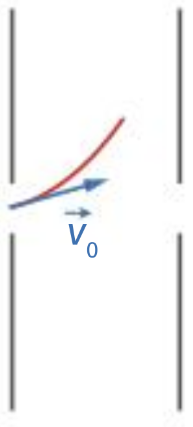
\includegraphics[scale=.3]{Ressources/TSPE_C5_EX_Fig5.png}
\end{center}
\end{minipage}
\begin{enumerate}
	\item Représenter le champ électrique $\vec{E}$ et le vecteur accélération $\vec{a}$ de la particule.
	\item Indiquer le signe des charges de chacune des plaques.
	\item Définir la trajectoire si le vecteur $\vec{v_0}$ était perpendiculaire aux plaques.
	\item Préciser quelle serait la trajectoire avec une particule chargée négativement.
\end{enumerate}
\end{multicols}
\end{document}
